\section{Cross Sectional Estimation Techniques}
\subsection{Some notes}
\begin{figure}[!ht]
	\centering
	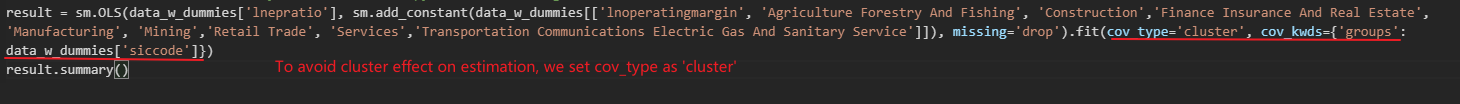
\includegraphics[width=\textwidth]{5/cluster.png}
\end{figure}
\begin{figure}[!ht]
	\centering
	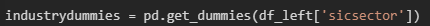
\includegraphics[width=\textwidth]{5/get_dummies.png}
\end{figure}
\begin{figure}[!ht]
	\centering
	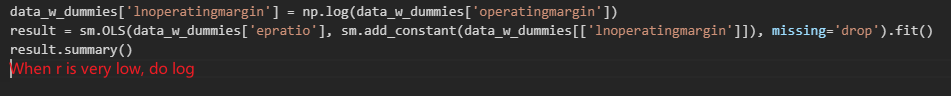
\includegraphics[width=\textwidth]{5/log.png}
\end{figure}
\begin{figure}[!ht]
	\centering
	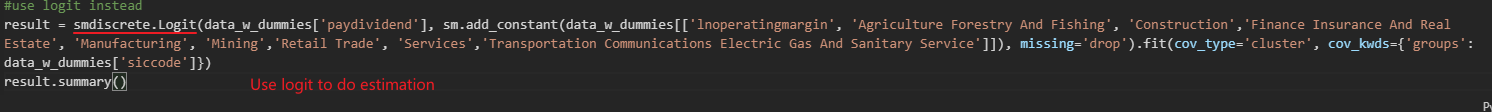
\includegraphics[width=\textwidth]{5/Logit.png}
\end{figure}
\begin{figure}[!ht]
	\centering
	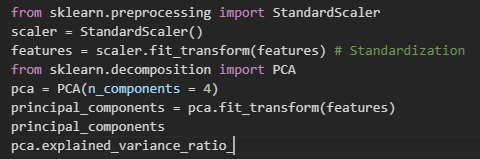
\includegraphics[width=\textwidth]{5/PCA.png}
\end{figure}

\begin{remark}
    Some key words: Fixed effects: dummy variables; t-statistic low: log; intra-cluster correlations: clustering; Collinearity: PCA; adding squared term; Hazard model; survival analysis 
\end{remark}